%  Make this into a pdf document as follows:
%
%
% The edit the Report.tex file appropriately to include only those elements that
% make sense for the assignment you're reporting on.
%
% You can use a tool like TeXShop or Texmaker or some other graphical tool
% to convert Report.text into a pdf file.
%
% If you are making this with command line tools, you'd run the following command:
%
%     latex Report.tex
%
% That will generate a dvi (device independent) document file called Report.dvi
% The pages reported in the table of contents won't be correct, since latex only
% processes one pass over the document. To adjust the page numbers in the contents,
% run latex again:
%
%    latex Report.tex
%
% Then run
%
%   dvipdf Report.dvi
%
% to generate Report.pdf
%
% You can view this file to check it out by running
%
% xdg-open Report.pdf
%
% That's it.
  
\def\cvss(#1,#2,#3,#4,#5,#6,#7,#8,#9){
	\indent\textbf{CVSS Base Severity Rating: #9}  AV:#1 AC:#2 PR:#3 UI:#4 S:#5 C:#6 I:#7 A:#8}
  
\def\ttp(#1, #2, #3, #4, #5, #6){
   \indent\textbf{#1:} #2 \\
   \indent\indent\textbf{#3:} #4 \\
   \indent\indent\indent\textbf{#5:} #6 \\}

\documentclass[notitlepage]{article}

\usepackage{bibunits}
\usepackage{comment}
\usepackage{graphicx}
\usepackage{amsmath}
\usepackage{datetime}
\usepackage{numprint}

% processes above options
\usepackage{palatino}  %OR newcent ncntrsbk helvet times palatino
\usepackage{url}
\usepackage{footmisc}
\usepackage{endnotes}

\setcounter{secnumdepth}{3}
\begin{document}

\nplpadding{2}
\newdateformat{isodate}{
  \THEYEAR -\numprint{\THEMONTH}-\numprint{\THEDAY}}
  
\title{Penetration Test Ex08}
\author{Esteban Calvo}
\date{\isodate\today}

\maketitle

\tableofcontents

\newpage

\section{Technical Report}

  \subsection{Finding: \emph{User Credentials}}
  
	\subsubsection*{Severity Rating}
	    High Risk:	    
		\cvss(L,L,N,R,U,H,H,N,7.1)
		
  	\subsubsection*{Vulnerability Description}
  		A password spraying method was used to find a list of possible user credentials for the internal email address. With a list of
        common passwords and some OSInt, I was able to access user emails and log on to the company email of one employee.

  	\subsubsection*{Confirmation method}
  	    Open port 443 in the browser with the following name
\begin{verbatim}
https://172.70.184.3:443
\end{verbatim}

    and enter the credentials (not included for confidentiality)

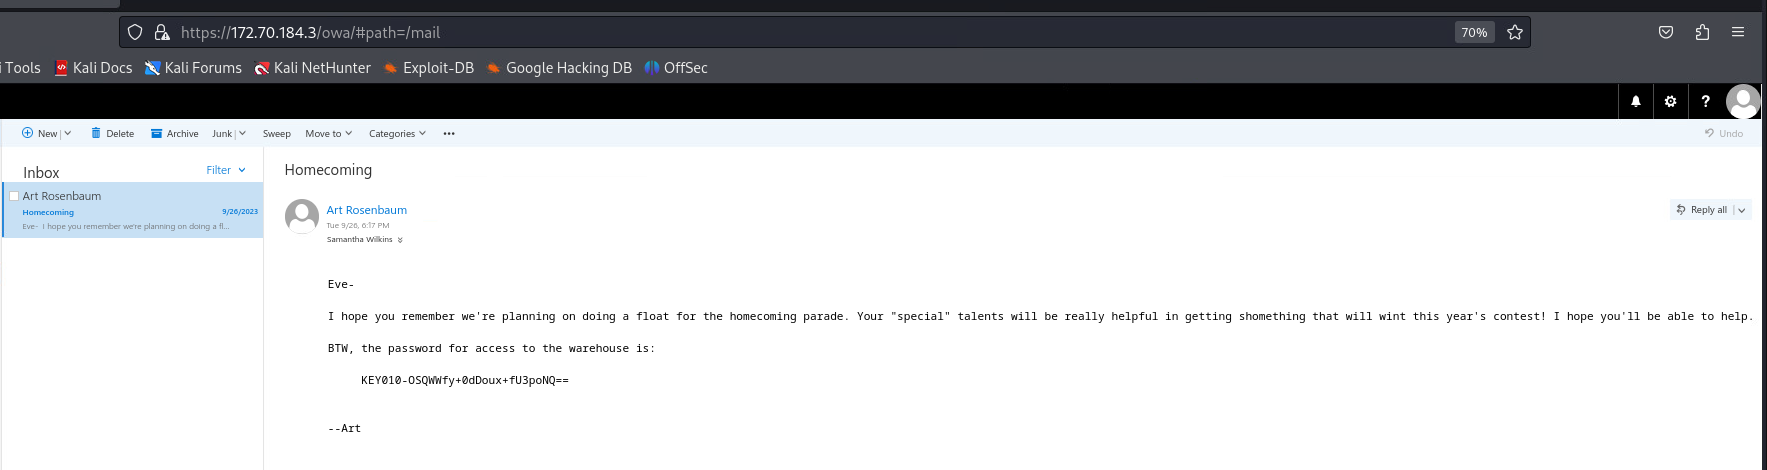
\includegraphics[width=5in]{~/Desktop/school/fall2023/pen/ex/ex08/outlook}
				
    \subsubsection*{Mitigation or Resolution Strategy}
        Have all employees change their passwords and have some sort of company program to check passwords against list of commonly used hashes and other forms of password validation.
        If it is too easy for attackers to guess the password, it will be inevitable that an attack can access sensitive user information. The use of MFA could also be enforced
        to ensure an attacker would need more than just one attack vector.



\section{Attack Narrative}
    
    \subsection{OSInt}
    To get a list of usernames, Google was used to find some possible credentials for some internal emails. Googling "Arts Tailor Shoppe" revealed a wiki with a
    list of superheroes and real names of some of the people Art makes costumes for. We are given the email "w.clockwell@artstailor.com", so I used this general structure
    with the list of superheros to compile a list of names that could be used. To generate the list of passwords, cewl as well as some generic commonly used passwords was used.
    The last step was putting it together and running the atomizer.py script as follows
    \begin{verbatim}
./atomizer.py owa https://mail.artstailor.com/owa/ passwords.txt users.txt --interval 0:0:1
    \end{verbatim}
    which revealed the credentials:
    \begin{verbatim}
user: artstailor\s.wilkins
password: Spring2023
    \end{verbatim}

    \subsection{Using Credentials to find Key}
    After using nmap on mail.artstailor.com, we found that there were 2 different ports open, 443 and 8443 as well as the innerouter IP of 172.70.184.3. Opening port 443 on the browser using the mail IP address, we were able to login
    to Samantha Wilkins email account. Once inside the email, I was able to see that there was only one email and this email as shown earlier included key 10. Once here, we also have access to send 
    emails and monitor new emails on her account until the password is changed.  \\
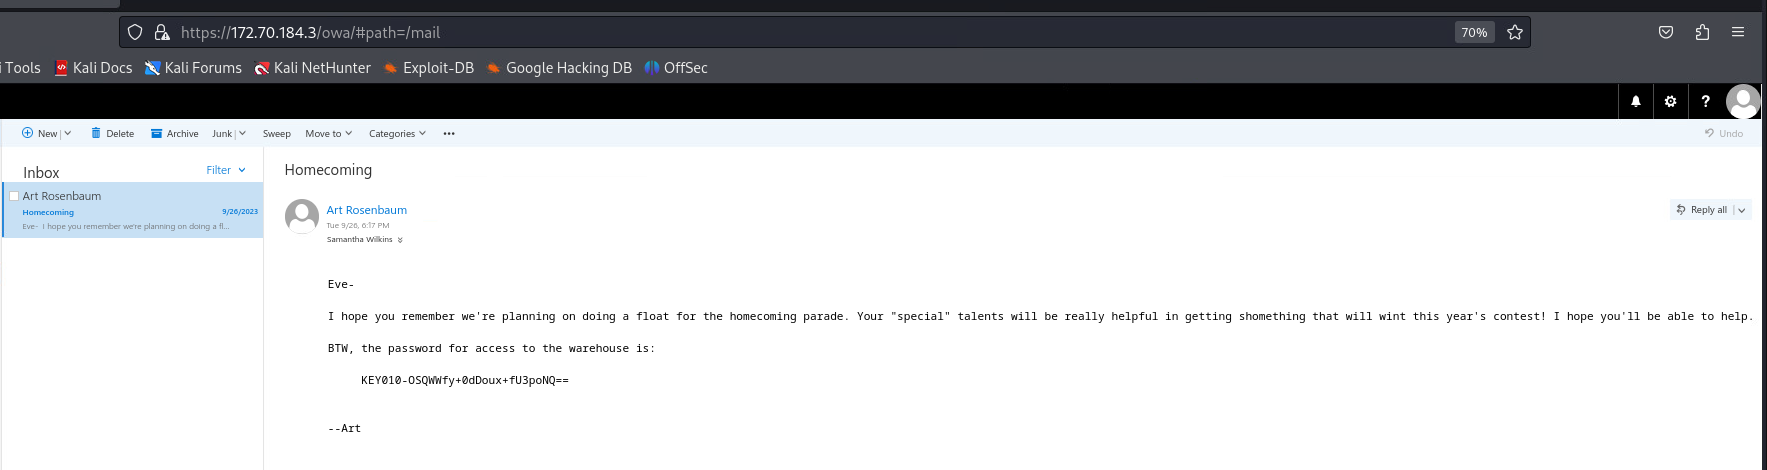
\includegraphics[width=5in]{~/Desktop/school/fall2023/pen/ex/ex08/outlook}

    \subsection{Port Forwarding}
    We are now able to open the other port we found available which was port 8443. On this port, we were able to access opnsense for artstailor innerouter. The default credentials still 
    seemed to work so using username root and password opnsense gave me access to write a new port forward for the network. Going to Firewall $\rightarrow$ NAT $\rightarrow$ Port Forwarding allowed me to forward
    the traffic coming in to innerouter to the RDP port in the machine 10.70.184.0/24. In one of the earlier assignments, we found some of IPs on this network that were open and in particular 
    the instructions mention costumes as being important so the router corresponding to costumes was used as follows: \\
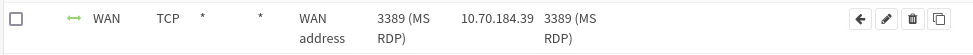
\includegraphics[width=5in]{~/Desktop/school/fall2023/pen/ex/ex08/portForward}
    From here, using the following command gave me access to a remote desktop on the RDP port and using the credentials found earlier gave me access Samantha's desktop
    \begin{verbatim}
rdesktop mail.artstailor.com
    \end{verbatim}
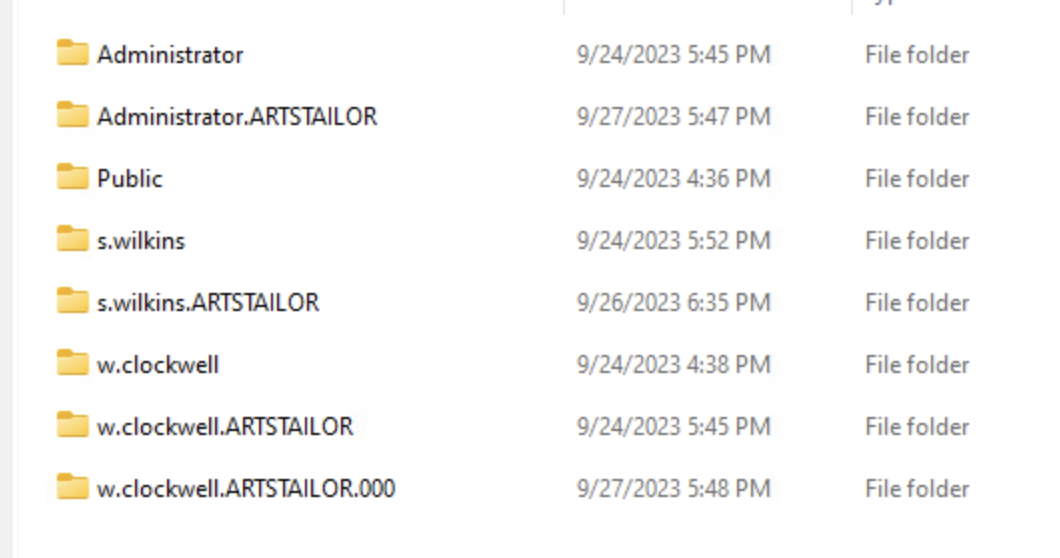
\includegraphics[width=5in]{~/Desktop/school/fall2023/pen/ex/ex08/desktop} \\

    \subsection{MITRE ATT{\&}CK Framework TTPs}
    \subsubsection*{}
    \ttp(TA0043, Reconnaissance, T1593, Search Open Websites/Domains, .002, Search Engine)
    
    \subsubsection*{}
    \ttp(TA0006, Credential Access, T1110, Brute Force, .003, Password Spraying)
    
    \subsection*{}
    \indent\textbf{TA0109:} Lateral Movement\\
    \indent\indent\textbf{T0812:} Default Credentials \\

    \subsection*{}
    \indent\textbf{TA0011:} Command and Control \\
    \indent\indent\textbf{T1572:} Protocol Tunneling \\

    \subsection{Temporary Internal Access to Artstailor}
    For the remainder of Penetration Testing, I would like access to the innerouter network. I feel it is important to gain access to the router for several reasons.
    I believe it is important for configuration review to make sure client facing ports such as seen with the buffer overflow incident are better guarded against. I also think
    it is important I can conduct more internal vulnerability scanning and access to internal services. Lastly, I want more ability to monitor router traffic and make sure that
    all people on the router have adequate credentials. To make sure my access is secure, ensure that there is strong authentication such as MFA and also make it to where users on this router
    must be on the internal network or using a VPN. 
\end{document} 
